% ##QuantumErrorCorrection
\documentclass[10pt,a4paper, english]{scrartcl}
\usepackage[utf8]{inputenc}
\usepackage{amsmath}
\usepackage{amsfonts}
\usepackage{amssymb}
\usepackage{babel}
\usepackage[cm]{fullpage}
\usepackage{float}
\usepackage{graphicx}
\usepackage{helvet}
\usepackage{hyperref}
\usepackage{mathtools}
\usepackage{nicefrac}
\usepackage{tikz}
\usepackage{pgfplots}
\usepackage{placeins}
\usepackage{verbatim}
\usepackage{xcolor}
\definecolor{gr}{gray}{0.9}
\renewcommand{\familydefault}{\sfdefault}
\title{Intro to Quantum Error Correction}
\author{Ben Criger}
\date{\today}
%    Q-circuit version 2
%    Copyright (C) 2004  Steve Flammia & Bryan Eastin
%    Last modified on: 9/16/2011
%
%    This program is free software; you can redistribute it and/or modify
%    it under the terms of the GNU General Public License as published by
%    the Free Software Foundation; either version 2 of the License, or
%    (at your option) any later version.
%
%    This program is distributed in the hope that it will be useful,
%    but WITHOUT ANY WARRANTY; without even the implied warranty of
%    MERCHANTABILITY or FITNESS FOR A PARTICULAR PURPOSE.  See the
%    GNU General Public License for more details.
%
%    You should have received a copy of the GNU General Public License
%    along with this program; if not, write to the Free Software
%    Foundation, Inc., 59 Temple Place, Suite 330, Boston, MA  02111-1307  USA

% Thanks to the Xy-pic guys, Kristoffer H Rose, Ross Moore, and Daniel Müllner,
% for their help in making Qcircuit work with Xy-pic version 3.8.  
% Thanks also to Dave Clader, Andrew Childs, Rafael Possignolo, Tyson Williams,
% Sergio Boixo, Cris Moore, Jonas Anderson, and Stephan Mertens for helping us test 
% and/or develop the new version.

\usepackage{xy}
\xyoption{matrix}
\xyoption{frame}
\xyoption{arrow}
\xyoption{arc}

\usepackage{ifpdf}
\ifpdf
\else
\PackageWarningNoLine{Qcircuit}{Qcircuit is loading in Postscript mode.  The Xy-pic options ps and dvips will be loaded.  If you wish to use other Postscript drivers for Xy-pic, you must modify the code in Qcircuit.tex}
%    The following options load the drivers most commonly required to
%    get proper Postscript output from Xy-pic.  Should these fail to work,
%    try replacing the following two lines with some of the other options
%    given in the Xy-pic reference manual.
\xyoption{ps}
\xyoption{dvips}
\fi

% The following resets Xy-pic matrix alignment to the pre-3.8 default, as
% required by Qcircuit.
\entrymodifiers={!C\entrybox}

\newcommand{\bra}[1]{{\left\langle{#1}\right\vert}}
\newcommand{\ket}[1]{{\left\vert{#1}\right\rangle}}
    % Defines Dirac notation. %7/5/07 added extra braces so that the commands will work in subscripts.
\newcommand{\qw}[1][-1]{\ar @{-} [0,#1]}
    % Defines a wire that connects horizontally.  By default it connects to the object on the left of the current object.
    % WARNING: Wire commands must appear after the gate in any given entry.
\newcommand{\qwx}[1][-1]{\ar @{-} [#1,0]}
    % Defines a wire that connects vertically.  By default it connects to the object above the current object.
    % WARNING: Wire commands must appear after the gate in any given entry.
\newcommand{\cw}[1][-1]{\ar @{=} [0,#1]}
    % Defines a classical wire that connects horizontally.  By default it connects to the object on the left of the current object.
    % WARNING: Wire commands must appear after the gate in any given entry.
\newcommand{\cwx}[1][-1]{\ar @{=} [#1,0]}
    % Defines a classical wire that connects vertically.  By default it connects to the object above the current object.
    % WARNING: Wire commands must appear after the gate in any given entry.
\newcommand{\gate}[1]{*+<.6em>{#1} \POS ="i","i"+UR;"i"+UL **\dir{-};"i"+DL **\dir{-};"i"+DR **\dir{-};"i"+UR **\dir{-},"i" \qw}
    % Boxes the argument, making a gate.
\newcommand{\meter}{*=<1.8em,1.4em>{\xy ="j","j"-<.778em,.322em>;{"j"+<.778em,-.322em> \ellipse ur,_{}},"j"-<0em,.4em>;p+<.5em,.9em> **\dir{-},"j"+<2.2em,2.2em>*{},"j"-<2.2em,2.2em>*{} \endxy} \POS ="i","i"+UR;"i"+UL **\dir{-};"i"+DL **\dir{-};"i"+DR **\dir{-};"i"+UR **\dir{-},"i" \qw}
    % Inserts a measurement meter.
    % In case you're wondering, the constants .778em and .322em specify
    % one quarter of a circle with radius 1.1em.
    % The points added at + and - <2.2em,2.2em> are there to strech the
    % canvas, ensuring that the size is unaffected by erratic spacing issues
    % with the arc.
\newcommand{\measure}[1]{*+[F-:<.9em>]{#1} \qw}
    % Inserts a measurement bubble with user defined text.
\newcommand{\measuretab}[1]{*{\xy*+<.6em>{#1}="e";"e"+UL;"e"+UR **\dir{-};"e"+DR **\dir{-};"e"+DL **\dir{-};"e"+LC-<.5em,0em> **\dir{-};"e"+UL **\dir{-} \endxy} \qw}
    % Inserts a measurement tab with user defined text.
\newcommand{\measureD}[1]{*{\xy*+=<0em,.1em>{#1}="e";"e"+UR+<0em,.25em>;"e"+UL+<-.5em,.25em> **\dir{-};"e"+DL+<-.5em,-.25em> **\dir{-};"e"+DR+<0em,-.25em> **\dir{-};{"e"+UR+<0em,.25em>\ellipse^{}};"e"+C:,+(0,1)*{} \endxy} \qw}
    % Inserts a D-shaped measurement gate with user defined text.
\newcommand{\multimeasure}[2]{*+<1em,.9em>{\hphantom{#2}} \qw \POS[0,0].[#1,0];p !C *{#2},p \drop\frm<.9em>{-}}
    % Draws a multiple qubit measurement bubble starting at the current position and spanning #1 additional gates below.
    % #2 gives the label for the gate.
    % You must use an argument of the same width as #2 in \ghost for the wires to connect properly on the lower lines.
\newcommand{\multimeasureD}[2]{*+<1em,.9em>{\hphantom{#2}} \POS [0,0]="i",[0,0].[#1,0]="e",!C *{#2},"e"+UR-<.8em,0em>;"e"+UL **\dir{-};"e"+DL **\dir{-};"e"+DR+<-.8em,0em> **\dir{-};{"e"+DR+<0em,.8em>\ellipse^{}};"e"+UR+<0em,-.8em> **\dir{-};{"e"+UR-<.8em,0em>\ellipse^{}},"i" \qw}
    % Draws a multiple qubit D-shaped measurement gate starting at the current position and spanning #1 additional gates below.
    % #2 gives the label for the gate.
    % You must use an argument of the same width as #2 in \ghost for the wires to connect properly on the lower lines.
\newcommand{\control}{*!<0em,.025em>-=-<.2em>{\bullet}}
    % Inserts an unconnected control.
\newcommand{\controlo}{*+<.01em>{\xy -<.095em>*\xycircle<.19em>{} \endxy}}
    % Inserts a unconnected control-on-0.
\newcommand{\ctrl}[1]{\control \qwx[#1] \qw}
    % Inserts a control and connects it to the object #1 wires below.
\newcommand{\ctrlo}[1]{\controlo \qwx[#1] \qw}
    % Inserts a control-on-0 and connects it to the object #1 wires below.
\newcommand{\targ}{*+<.02em,.02em>{\xy ="i","i"-<.39em,0em>;"i"+<.39em,0em> **\dir{-}, "i"-<0em,.39em>;"i"+<0em,.39em> **\dir{-},"i"*\xycircle<.4em>{} \endxy} \qw}
    % Inserts a CNOT target.
\newcommand{\qswap}{*=<0em>{\times} \qw}
    % Inserts half a swap gate.
    % Must be connected to the other swap with \qwx.
\newcommand{\multigate}[2]{*+<1em,.9em>{\hphantom{#2}} \POS [0,0]="i",[0,0].[#1,0]="e",!C *{#2},"e"+UR;"e"+UL **\dir{-};"e"+DL **\dir{-};"e"+DR **\dir{-};"e"+UR **\dir{-},"i" \qw}
    % Draws a multiple qubit gate starting at the current position and spanning #1 additional gates below.
    % #2 gives the label for the gate.
    % You must use an argument of the same width as #2 in \ghost for the wires to connect properly on the lower lines.
\newcommand{\ghost}[1]{*+<1em,.9em>{\hphantom{#1}} \qw}
    % Leaves space for \multigate on wires other than the one on which \multigate appears.  Without this command wires will cross your gate.
    % #1 should match the second argument in the corresponding \multigate.
\newcommand{\push}[1]{*{#1}}
    % Inserts #1, overriding the default that causes entries to have zero size.  This command takes the place of a gate.
    % Like a gate, it must precede any wire commands.
    % \push is useful for forcing columns apart.
    % NOTE: It might be useful to know that a gate is about 1.3 times the height of its contents.  I.e. \gate{M} is 1.3em tall.
    % WARNING: \push must appear before any wire commands and may not appear in an entry with a gate or label.
\newcommand{\gategroup}[6]{\POS"#1,#2"."#3,#2"."#1,#4"."#3,#4"!C*+<#5>\frm{#6}}
    % Constructs a box or bracket enclosing the square block spanning rows #1-#3 and columns=#2-#4.
    % The block is given a margin #5/2, so #5 should be a valid length.
    % #6 can take the following arguments -- or . or _\} or ^\} or \{ or \} or _) or ^) or ( or ) where the first two options yield dashed and
    % dotted boxes respectively, and the last eight options yield bottom, top, left, and right braces of the curly or normal variety.  See the Xy-pic reference manual for more options.
    % \gategroup can appear at the end of any gate entry, but it's good form to pick either the last entry or one of the corner gates.
    % BUG: \gategroup uses the four corner gates to determine the size of the bounding box.  Other gates may stick out of that box.  See \prop.

\newcommand{\rstick}[1]{*!L!<-.5em,0em>=<0em>{#1}}
    % Centers the left side of #1 in the cell.  Intended for lining up wire labels.  Note that non-gates have default size zero.
\newcommand{\lstick}[1]{*!R!<.5em,0em>=<0em>{#1}}
    % Centers the right side of #1 in the cell.  Intended for lining up wire labels.  Note that non-gates have default size zero.
\newcommand{\ustick}[1]{*!D!<0em,-.5em>=<0em>{#1}}
    % Centers the bottom of #1 in the cell.  Intended for lining up wire labels.  Note that non-gates have default size zero.
\newcommand{\dstick}[1]{*!U!<0em,.5em>=<0em>{#1}}
    % Centers the top of #1 in the cell.  Intended for lining up wire labels.  Note that non-gates have default size zero.
\newcommand{\Qcircuit}{\xymatrix @*=<0em>}
    % Defines \Qcircuit as an \xymatrix with entries of default size 0em.
\newcommand{\link}[2]{\ar @{-} [#1,#2]}
    % Draws a wire or connecting line to the element #1 rows down and #2 columns forward.
\newcommand{\pureghost}[1]{*+<1em,.9em>{\hphantom{#1}}}
    % Same as \ghost except it omits the wire leading to the left. 

\usepackage{amsmath}
\usepackage{bbold}
\usepackage{color}
\usepackage{stmaryrd}
\usepackage{calc}
\usepackage{verbatim}
\usepackage{mathtools}
\usepackage{xspace}
\DeclarePairedDelimiter{\ceil}{\lceil}{\rceil}
\DeclarePairedDelimiter{\floor}{\lfloor}{\rfloor}
\usepackage{tikz}
\usetikzlibrary{calc}
\providecommand{\polygon}[2]{%
  let \n{len} = {2*#2*tan(360/(2*#1))} in
 ++(0,-#2) ++(\n{len}/2,0) \foreach \x in {1,...,#1} { -- ++(\x*360/#1:\n{len})}}

\DeclareMathOperator\erf{erf}
\DeclareMathOperator\erfc{erfc}

\newsavebox\CBox
\newcommand\hcancel[2][0.5pt]{%
  \ifmmode\sbox\CBox{$#2$}\else\sbox\CBox{#2}\fi%
  \makebox[0pt][l]{\usebox\CBox}%  
  \rule[0.5\ht\CBox-#1/2]{\wd\CBox}{#1}}

\providecommand{\drv}[1]{\dfrac{\partial }{\partial #1}}
\providecommand{\drf}[2]{\dfrac{\partial #1}{\partial #2}}
\providecommand{\ddrf}[3]{\dfrac{\partial^2 #1}{\partial #2 \partial #3}}

\providecommand{\tr}{\mathrm{tr}}
 
\providecommand{\ket}[1]{\left \vert #1 \right \rangle}
\providecommand{\bra}[1]{\left \langle #1 \right \vert}
\providecommand{\braket}[2]{\left \langle #1 \left \vert #2 \right. \right \rangle}
\providecommand{\angles}[1]{\left \langle #1 \right \rangle}
\providecommand{\elem}[3]{\left \langle #1 \left \vert \vphantom{#1#2#3} #2 \right \vert #3 \right \rangle}
\providecommand{\delem}[2]{\left \langle #1 \left \vert \vphantom{#1#2} #2 \right \vert #1 \right \rangle}
\providecommand{\ketbra}[2]{\ket{#1} \! \bra{#2}}
\providecommand{\proj}[1]{\ketbra{#1}{#1}}
\providecommand{\twonorm}[1]{\| #1 \|_2}
\providecommand{\abs}[1]{\left \vert #1 \right \vert}
\providecommand{\set}[1]{\left \lbrace #1 \right \rbrace}
\providecommand{\group}[1]{\left \langle #1 \right \rangle}
\providecommand{\red}[1]{\textcolor[rgb]{0.5,0,0}{#1}}
\providecommand{\blue}[1]{\textcolor[rgb]{0,0,0.5}{#1}}
\providecommand{\green}[1]{\textcolor[rgb]{0,0.5,0}{#1}}
\providecommand{\conjecture}[1]{\red{#1 (check this).}}
\providecommand{\future}[1]{\green{#1 (do this later).}}
\providecommand{\id}{\hat{\mathbb{1}}}
\providecommand{\com}[2]{\left[#1,\,#2 \right]}
\providecommand{\acom}[2]{\left \lbrace #1,\,#2 \right \rbrace}
\providecommand{\diss}[2]{\mathcal{D}\left[ #1 \right]\left( #2 \right)}
\providecommand{\meas}[2]{\mathcal{M}\left[ #1 \right]\left( #2 \right)}
\providecommand{\lindtwo}[2]{ #1 #2 #1^{\dagger} - \dfrac{1}{2} \left \lbrace #1^{\dagger} #1,\,#2 \right \rbrace }
\providecommand{\lindthree}[3]{ #1 #2 #3 - \dfrac{1}{2} \acom{#3 #1}{#2} }
\providecommand{\lindfour}[4]{ #1 #2 #3 - \dfrac{1}{2} \acom{#4}{#2} }
\providecommand{\meastwo}[2]{ #1 #2 + #2 #1^{\dagger} - \tr \left( #1 #2 + #2 #1^{\dagger} \right) #2 }
\providecommand{\tenscom}[4]{\com{#1\otimes #2}{#3 \otimes #4}=\dfrac{1}{2}\left( \com{#1}{#3} \otimes \acom{#2}{#4} + \acom{#1}{#3} \otimes \com{#2}{#4} \right)}
\providecommand{\tenscomsimple}[4]{\com{#1\otimes #2}{#3 \otimes #4} = #1 #3 \otimes \com{#2}{#4} + \com{#1}{#3} \otimes  #4 #2}
\providecommand{\tensacom}[4]{\acom{#1\otimes #2}{#3 \otimes #4}=\dfrac{1}{2}\left( \com{#1}{#3} \otimes \com{#2}{#4} + \acom{#1}{#3} \otimes \acom{#2}{#4} \right)}
\providecommand{\trace}[1]{\mathrm{tr} \left( #1 \right)}
\providecommand{\comp}{\mathop{\bigcirc}}
\providecommand{\swap}{\textsc{swap}\xspace}
\providecommand{\cnot}{\textsc{cnot}\xspace}
\providecommand{\col}{\textrm{col}}
\providecommand{\qec}[3]{\llbracket #1,\,#2,\,#3 \rrbracket}
\providecommand{\set}[1]{\left \lbrace #1 \right \rbrace}
\renewcommand{\Im}{\textrm{Im}}
\renewcommand{\Re}{\textrm{Re}}
\providecommand{\lind}{\mathcal{L}}
\providecommand{\norm}[2]{\left \vert \left \vert #2 \right \vert \right \vert_{#1}}
\providecommand{\supp}[1]{\mathrm{supp}\left( #1 \right)}
\providecommand{\given}{\, \middle \vert \,}
\providecommand{\suchthat}{\, \middle \vert \,}
\providecommand{\diag}[1]{\mathrm{diag}\left( #1 \right)}
\providecommand{\ct}{^{\dagger}}

\providecommand{\norm}[1]{\left\Vert #1 \right\Vert} %only works with amsmath

\providecommand{\ncrit}{$n_{\textrm{crit}}$\xspace}

\makeatletter
\providecommand{\pr}[2]{p\left(#1\,\middle|\,#2\right)}
\newcommand{\pushright}[1]{\ifmeasuring@#1\else\omit\hfill$\displaystyle#1$\fi\ignorespaces}
\newcommand{\pushleft}[1]{\ifmeasuring@#1\else\omit$\displaystyle#1$\hfill\fi\ignorespaces}
\makeatother
\newlength\figureheight
\newlength\figurewidth
\setlength\figureheight{7cm}
\setlength\figurewidth{12cm}

\providecommand{\cnot}{\textsc{cnot}}
\providecommand{\volts}{\, \textrm{V}}

\usetikzlibrary{decorations.pathreplacing,decorations.pathmorphing}

\begin{document}
\maketitle
\section{Introduction}
The purpose of this note is to help introduce quantum error correction [QEC] and (especially) fault-tolerance to people who are not familiar with quantum mechanics, or quantum computing, such as:
\begin{itemize}
\item undergraduates,
\item electrical/computer/software engineers,
\item experimental physicists now trying to implement QEC, who have missed such an introduction.
\end{itemize}
My goals in writing this note are:
\begin{itemize}
\item to keep it short, at the cost of completeness,
\item to refer to longer/superior works where possible (often),
\item to frequently compare ``scary quantum'' processes with their classical equivalents, to help de-mystify QEC.
\end{itemize}
[Insert usual caveat about imprecise notation, i.e.: these notes are free, and you get what you pay for.]

I begin in the following section with an explanation of why error correction is necessary, moving on to describe the difference between error-correction and fault-tolerance, before moving on to the most popular elements of QEC theory (stabilizer codes $\mapsto$ CSS codes $\mapsto$ homological codes $\mapsto$ the surface code). 
\section{Why Error Correction?}
If you meet a software engineer in the street, the need for error correction may not be obvious. 
In the life of a computer programmer, errors are things caused exclusively by people, and careful thinking and good practices are required to prevent, detect and correct them. 
[Maybe there's a repetition code at work here, especially with \texttt{diff}, but that is an analogy for another day.]
However, if you scratch the surface, you find instances of error correction and even (what I'm going to call) fault-tolerance at work. 

Take, for example, satellite/spacecraft communications. 
These spacecraft are very far away, and there are bits that don't make it between the spacecraft and the ground station. 
Actually, that example is too far outside our daily experience to take, so let's take flash drives, AKA USB keys.
The job of these drives is to store bits ($0$'s and $1$'s), which they manage to do most of the time.
However, one bit in every $10^{4\text{--}9}$ is randomly flipped, which in the worst case scenario would lead to an ASCII typo per page of text [or something].

To compensate for this, the USB key records the information redundantly, using more bits than are strictly necessary.
When reading, the CPU can then check that different decodings of the redundant information are consistent, and if they're not, can infer a decoding that's likely to be correct. 
The fact that the CPU is not itself (assumed to be) error-prone is a great boon to us in reading USB keys, otherwise we couldn't trust that any decoding was correct. 

There's a reason that CPUs are not considered noisy, by the way.
Transistor-transistor logic (TTL for short) defines a standard voltage for its $0$ and $1$ states, usually $0 \volts$ and  $5 \volts$, respectively.
These circuits can be designed to output $0 \volts$ for any input voltage between $0 \volts$ and $0.4 \volts$, likewise to output $5 \volts$ whenever a voltage of $2.6 \volts$ or higher is input. 
This is a (very powerful) error correction mechanism. 
If noise spreads voltages out according to some unimodal distribution, we can tighten that distribution at every TTL element, paying only a small energy cost to do so. 
In theory, we could also design an element which outputs a third value whenever the input voltage doesn't correspond to a logical $0$ or $1$, so that we can detect errors. 
In practice, we would just increase the supply voltage until we don't have to worry. 

The availability of reliable components which can be used to store and process classical information is a great benefit to computer engineers.
In the following sections, we'll see which of these properties can also be achieved for quantum systems. 
But first, some definitions.
\subsection{What is a Code?}
A code is a subset. 

If you have a system, classical quantum or other, which can assume states from some set, you can define any subset of these states to be a code.
The states in the code are called the \emph{codewords}.

Most of the time, we will also constrain our codes to be \emph{linear} with respect to some operation (usually denoted $+$), which means that for any codewords $a$ and $b$, $a + b$ is also a codeword. 
This is pretty common, and it means we can normally consider state sets which are vector spaces, and codes which are subspaces. 
This is true in both the classical and quantum case. 

A code can be used to fulfil a variety of purposes.
Compression, for example, involves codes whose codewords are shorter than the logical messages they represent.

We will mostly concern ourselves with \emph{error-correcting} codes, which can only be analysed using two other mathematical objects as tools.
The first of these is the \emph{error model}, the set of possible transformations which can act on a state (codeword or otherwise) without our knowledge. 
The second is the \emph{recovery map}, which takes as input states from the full set and outputs corresponding codewords. 
To solidify these ideas, let's consider an example.
\subsubsection{Example: 3-Bit Repetition Code}
Suppose Alice wants to tell Bob the value of a bit, $0$ or $1$, but that she has to use a channel which is subject to symmetric bit-flip:
\begin{figure}[!h]
\centering
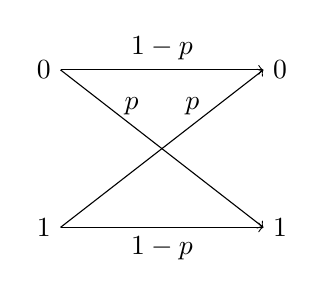
\begin{tikzpicture}[x=3cm, y=2cm]
\node (in0) at (0, 1) {$0$};
\node (in1) at (0, 0) {$1$};
\node (out0) at (1, 1) {$0$};
\node (out1) at (1, 0) {$1$};
\draw [->] (in0.east) -- (out0.west) node [above,align=center,midway] {$1-p$};
\draw [->] (in0.east) -- (out1.west) node [above,align=center,pos=0.35] {$p$};
\draw [->] (in1.east) -- (out0.west) node [above,align=center,pos=0.65] {$p$};
\draw [->] (in1.east) -- (out1.west) node [below,align=center,midway] {$1-p$};
\end{tikzpicture}
\caption{Graphical representation of an error map on a classical bit which flips the bit (taking $0$ to $1$ and vice versa) with probability $p$.}
\end{figure}

Alice, then, would like to send messages from $\mathbb{Z}_2$, so she should design codes that have two codewords. 
Supposing that Alice has repeated access to the channel, and knows the probability $p$, she can design codes which use $\mathbb{Z}_2^n$ as the full state space. 
A simple thing that Alice can do is repeat herself three times (taking $n=3$) to make herself understood.
Bob, then, should infer that $0$ is the desired message when he receives a state containing mostly $0$s and $1$ when he receives a state containing mostly $1$s. 
Let's express these ideas mathematically, so that we can generalize later.

\begin{description}
\item[Codewords]: $000$, $111$
\item[Error Model]:
\begin{equation}
000 \mapsto \begin{array}{cl}
000 & (1-p)^3 \\ 001,\, 010,\, 100 & p(1-p)^2 \\ 110,\, 101,\, 011 & p^2(1-p) \\ 111 & p^3
\end{array} \quad 
111 \mapsto \begin{array}{cl}
111 & (1-p)^3 \\ 110,\, 101,\, 011 & p(1-p)^2 \\ 001,\, 010,\, 100 & p^2(1-p) \\ 000 & p^3
\end{array}
\end{equation} 
\item[Recovery Map]: $(000,\,001,\,010,\,100) \mapsto 000$, $(111,\,110,\,101,\,011) \mapsto 111$
\end{description}
We can see that, if there is a weight-two or weight-three error, Bob will infer the incorrect state.
The resulting probability of error is $3p^2(1-p) + p^3$. 

\textbf{Exercise: } When does this protocol amplify errors? How should we remedy this?

We will go on to construct quantum codes in later sections. 
But first, I should confess something.
\subsection{Fault Tolerance}
Let's begin with an overall reminder of what we're trying to accomplish.
We want to replicate the properties of TTL logic for quantum states and operations.
Not only are we able to interpret the output of a TTL gate using a perfect computer, we also know that TTL operations suppress errors that occur \emph{during the operations themselves}. 
We therefore have to \emph{encode operations} in some way, using a small subset of operations drawn from some large set to ensure that errors from the operations used to correct the code can themselves be corrected. 
For the first few examples, we won't focus on this, since it's useful to see that we can correct `vanilla' errors before moving on to attempt fault tolerance.

\section{Quantum Codes}
If fault tolerance wasn't a big enough problem, we have another one. 
Error models for quantum systems are much more complex than those for classical bits, because they're \emph{continuous}. They don't map $\ket{\psi}$ to $\ket{\psi_{\perp}}$, but instead to $U\ket{\psi}$ for $U$ some unknown unitary, for example.
There are even some channels for which no mixture of unitaries can describe the channel's effects. 
For this general set of quantum channels, we can represent their effects mathematically using a set of operators. 
This is frequently called the \emph{Kraus representation}, after Karl Kraus. 
Given these operators (let's call them $E_j$), we calculate the effect of the channel on a density matrix as follows:
\begin{equation}
\rho \mapsto \sum_j E_j \rho E_j \ct
\end{equation}
There's also a constraint on these operator sets.
In order to be valid transformations on quantum states, they have to map density matrices to density matrices.
Since density matrices are positive-semidefinite with trace one, the action of the operator set must be \emph{completely positive} (preserving positivity, even when it acts on \emph{part of a larger system}), and trace-preserving. 
This is true iff $\sum_j E_j \ct E_j = \id$.
Let's get this clearer with an example. 
Let's do bit-flip again, calling the channel $B$:
\begin{flalign}
B_0 = \sqrt{1 - p} \begin{bmatrix}
1 & 0 \\ 0 & 1
\end{bmatrix}, \quad B_1 = \sqrt{p} \begin{bmatrix}
0 & 1 \\ 1 & 0 
\end{bmatrix}
\end{flalign}
We can calculate the effect on a one-qubit density matrix with ground state population $q$ and coherence $c$:
\begin{flalign}
\rho &= \begin{bmatrix}
q & c \\ c^\ast & 1-q
\end{bmatrix} \\
\sum_j B_j \rho B_j \ct &= (1 - p) \rho + p X \rho X \\
&= (1 - p) \begin{bmatrix}
q & c \\ c^\ast & 1-q
\end{bmatrix}
 + p \begin{bmatrix}
   1-q & c^\ast \\c & q
\end{bmatrix} \\
&= \begin{bmatrix}
q + p - 2pq & c - p (c - c^\ast) \\
c^\ast - p (c^\ast - c) & 1 - p - q + 2pq
\end{bmatrix}
\end{flalign}
\textbf{Exercise: } Sub in the $\ket{0}$ and $\ket{1}$ states. What happens to them?

If we allow generic operations, this looks similar to the central problem of analog computing, that it's far easier to force an input from a continuous space to a few discrete values (oh, say, $0 \volts$ and $5 \volts$) than it is to force noisy values to stay close to the value that some arbitrary computation should be at ($x \volts$). 
For this reason, people with experience in analog computing are wary of quantum computing when they hear about it. 
All is not lost, though. 
In the next subsection, we'll see that these analog errors can be \emph{digitized}, but first, we have to define what it means to correct an error in the quantum case.
\subsection{The Knill-Laflamme Criterion and Noise Digitization}
To talk about which quantum errors can be corrected, we should first make clear that in the typical case, not all of them can be corrected. 
To see this, consider the quantum bit-flip map defined above, and its action on the quantum bit-flip code $\ket{000},\,\ket{111}$.
With probability $p^3$, the channel maps one logical state directly to the other. 
Any sane recovery map would include $\ket{111} \mapsto \ket{111}$, so that there's always some probability of error. 
However, we can always try to take a subset of the operators $E_j$ and declare it to be exactly correctable. 
If our codewords are labeled $\ket{\psi_j}$, then this happens whenever
\begin{equation}
\elem{\psi_j}{E_k\ct E_l}{\psi_m} = C_{kl} \delta_{jm}
\end{equation}
Due to limited time, we won't go through the proof, but a detailed and accessible proof can be found in section 2.3 of Lidar and Brun. 
I would like to focus on the interpretation of this formula instead. 
First, let's note that it implies that any time two different codewords are acted upon by correctable Kraus operators, the resulting states will still be orthogonal. 
This means that, in theory, a recovery map can be designed which maps them back to the original code states, though this may be difficult in practice. 

Second, and more importantly, it implies that if a code can correct two Kraus operators $E_a$ and $E_b$, it can correct any linear combination of the two.
I will also not prove this, but it's in section 2.6 of Lidar/Brun.
If we can correct an $X$, $Y$ or $Z$ error on an arbitrary qubit, though, it follows that we can correct any single-qubit error, since $X$, $Y$, and $Z$ form a basis for the set of possible operators on one qubit.
It takes a little work to get such a code, we'll see some examples in the next section. 
\subsection{The Nine-Qubit Code}
\subsection{The Five-Qubit Code}
This motivates the introduction of some new formalism, to make sure that the codes we study don't require us to write down an exponential number of parameters.
\section{The Stabilizer Formalism in a Nutshell}
There is at least one well-studied way to do this (there are a few others as well, but they're not as popular).
This theory uses operators instead of quantum states as its representation, because tensor-product operators can give rise to states with non-trivial entanglement, which it turns out is necessary to do error correction [Prove this?].
This is the so-called \emph{Heisenberg picture}. 

It's also best to use operators that form a group to do this, that way we don't have to keep track of any matrices during a calculation, we can just use the group operation. 
Our operators have $+1$ and $-1$ eigenspaces of equal size [Prove this]. 
This means that, if we want to specify an $n-1$-qubit subspace of a space, we only have to write down one $n$-qubit operator, given as an $\mathcal{O}(n)$-letter string. 
This means that, in order to define a subspace with $k$ ``logical'' or ``effective'' qubits, 
we specify $n-k$ stabilisers, using a total of $\mathcal{O}(n^2)$ letters (assuming $k$ doesn't scale with $n$).

It remains to be seen that subspaces defined in this way can detect/correct errors.
Let's show that Pauli errors can be detected if they anticommute with some stabiliser, and that a set can be corrected if any two such errors don't form a logical when you multiply them.
[Go ahead and show that].
\subsection{CSS codes}
These are like easy stabiliser codes.
\subsection{Homological Codes}
These are like easy CSS codes.
\subsection{The Surface Code}
This is like an easy homological code.
\end{document}